
With this snapshot program, we propose to use HST's WFC3-IR detector
to discover the first multiply-imaged SN behind a strong lensing
galaxy cluster, setting the gold standard for future strong lensing
time delay measurements.  In recent years HST programs such as CLASH
and the Hubble Frontier Fields have built up a deep trove of WFC3-IR
imaging on strong-lensing galaxy clusters at redshifts $z\sim0.5$.
Many of these clusters have dozens of multiply-imaged background
galaxies at redshifts $1\lesssim z \lesssim 6$, which have been used
to produce well-constrained models of the cluster lensing potential.
When a SN inevitably appears within one of these multiply-imaged
galaxies, it will of course be multiply-imaged itself.  With that SN
we could measure a time delay distance with better than 6\%
precision, providing a unique and powerful
constraint on \Ho\ and dark energy.  With deep template imaging for
over 25 rich clusters in hand, {\bf \em we now have a viable pathway
to discover the first ever multiply-imaged SN with a small, single-cycle
snapshot program.}


\medskip
\noindent {\bf Time Delay Cosmography}

As light from a distant source passes through a galaxy cluster,
strong gravitational lensing causes multiple images to appear to the
observer, with a time separation between the images given by


\vspace{-5mm}
\begin{tabular}{p{5.5cm}r}
% \dt = \frac{\Dl \Ds}{\Dls} ( 1 + z_l ) \phi
{\begin{align}
%\begin{equation}\label{eq:dt}
 %  \dt = \frac{\Dl \Ds}{\Dls} ( 1 + z_l ) \phi
%\end{equation}
  \dt &= \frac{\Dl \Ds}{c\,\Dls} ( 1 + z_L ) \phi \label{eq:dt} \\
  \phi &= \frac{1}{2}(\theta-\beta)^2 - \psi(\theta) \label{eq:phi}
\end{align}}
&
\hspace{1cm}
\raisebox{-30mm}{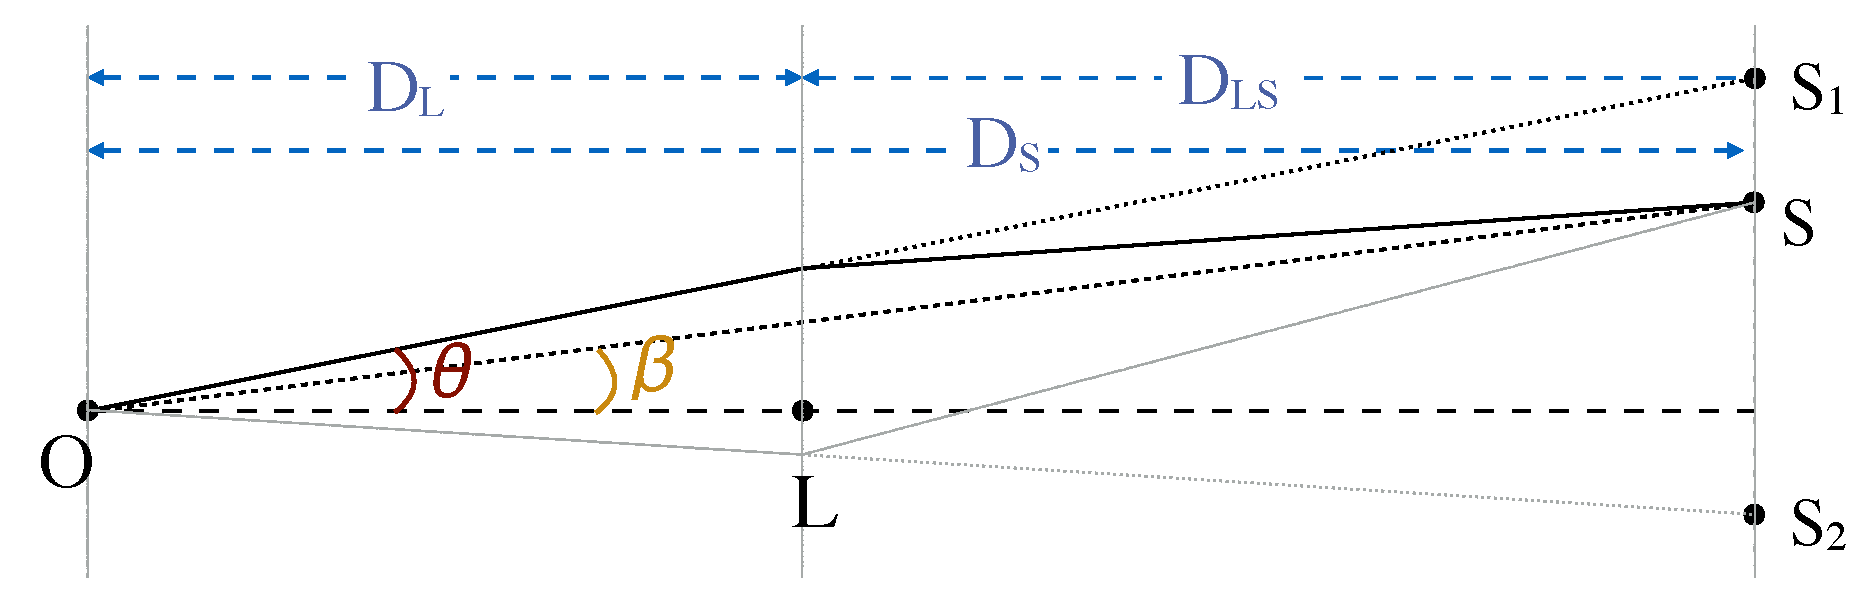
\includegraphics[width=0.5\textwidth]{FIG/lensingGeometry2}}
%\raisebox{-30mm}{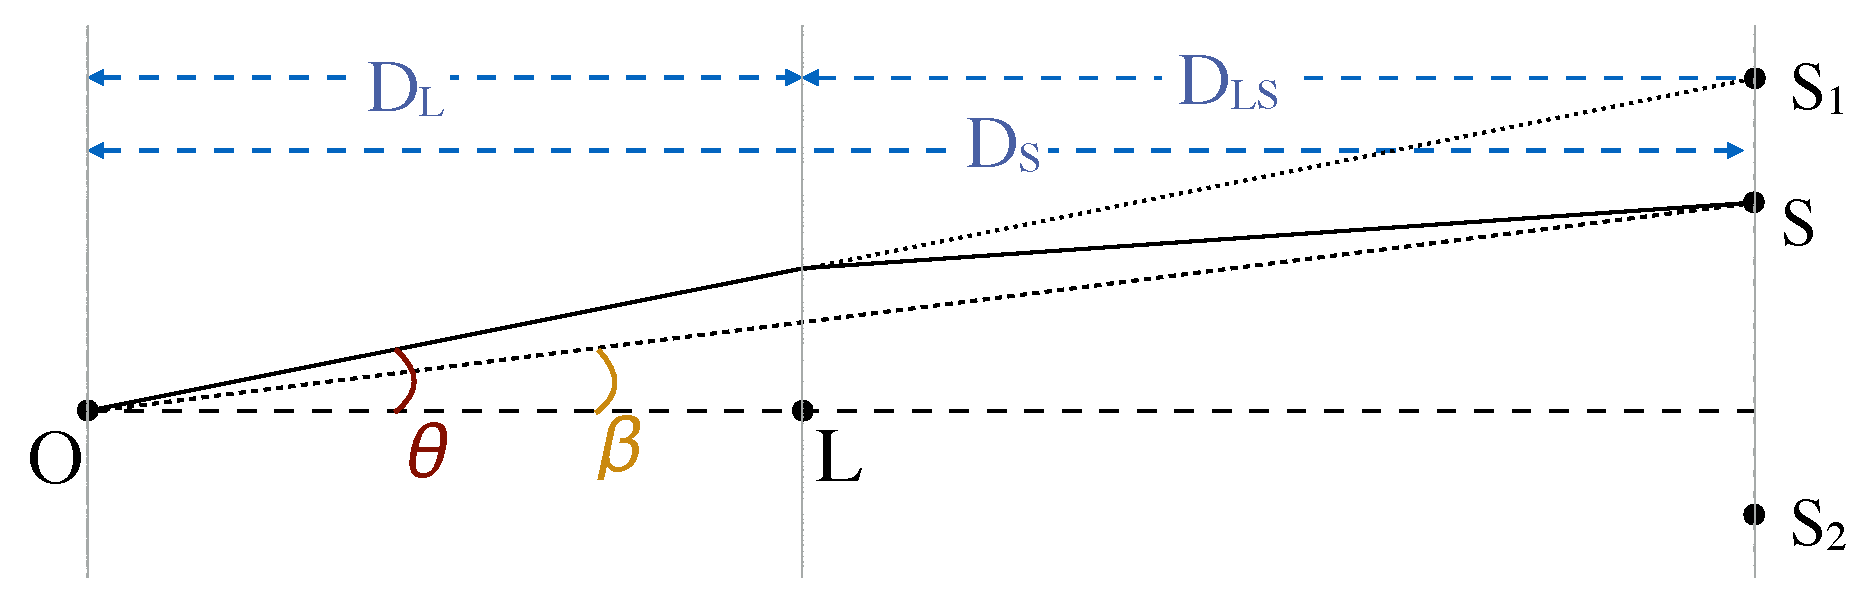
\includegraphics[width=0.5\textwidth]{FIG/lensingGeometry}}
\end{tabular}


\noindent where the redshift of the lens is $z_L$, while \Dl, \Ds, 
and \Dls\ are angular diamater distances from the observer to the
lens, observer to source, and lens to source, respectively.  The time
delay potential, $\phi$, is given in Eq.~\ref{eq:phi}. The first term
gives the geometric delay due to light rays following different path
lengths to the observer, and the second term, $\psi$, is the
relativistic component due to differing values of the gravitational
potential along each path.

Each of the distances in Equation~\ref{eq:dt} carries a factor
of \Ho$^{-1}$, so if the lensing potential $\phi$ is well known, then a
time delay measurement provides a direct measurement of the Hubble
constant.  The distance ratio $\Dl\Ds/\Dls$ also has
unusual sensitivities to cosmological parameters as a function of
redshift that make this technique a particularly useful probe of
dynamic dark energy models \citep{Linder:2011}.

\citet{Refsdal:1964} first proposed the use of SN time delays as 
a means to measure \Ho.  Now 50 years later, this has not yet been
achieved, primarily due to the small number of very well analyzed
gravitational lenses ($\sim$dozens), and the short visibility window
for any given high-$z$ SN event ($\sim$a few weeks).  Only recently
have we begun to realize the potential in this technique with the
recent measurement of a few dozen time delays of quasars, being lensed
typically by a single foreground galaxy \citep{Jackson:2007}. Among
these, only a handful have time delays measured with particularly high
precision \citep[e.g.]{Suyu:2010,Suyu:2013}.  These quasar lenses
generally suffer from a number of serious concerns, notably: (1) the
lensing potential is poorly constrained due to inherent degeneracies
and insufficient constraints; (2) the time delays and angular
separations are quite small (tens of days, fractions of an arcsecond);
and (3) the source is continuously variable, requiring many years of
stable monitoring to resolve phase degeneracies.  Wide-field surveys
in the coming decade could deliver $>$100 quasar time delays, but
these problems represent unavoidable systematic biases for this
sample.


\medskip
\noindent {\bf The SN Time Delay Advantage}
 
In Cycle 22, HST has just achieved a new capability for the discovery
of a strongly-lensed SN. The first key advancement was the
availability of WFC3-IR, which allows HST imaging surveys to capture
high-$z$ SN at the peak of their SED profile in rest-frame optical
bands \citep{Rodney:2012,Jones:2013}.  Ground-based surveys and even
HST/ACS programs have searched for multiply-imaged SN in the past, but
none have had the capability to detect even highly magnified SN at
$z>2$ \citep[e.g.][]{Dawson:2009,Sand:2011}.  With WFC3-IR, \Hubble\
now has access to a much larger survey volume with each pointing.

A WFC3-IR program targeting massive clusters, such as CLASH or the
Hubble Frontier Fields, could in principal have caught a strongly
lensed SN already, but in practice the likelihood of such a find was
vanishingly small.  The CLASH team collected WFC3-IR imaging of 25
clusters over 3-years, but the time separation between the first and
last image on any single cluster was never more than a few months.
However, these programs -- along with other WFC3-IR cluster imaging
campaigns -- have now provided the second critical advance: deep IR
template imaging of massive clusters from which to construct
difference images for SN discovery.  These HST programs have also led
to an explosion of detailed mass modeling for strong-lensing clusters,
providing well-defined lensing potentials that will be crucial for
evaluating a multiply-imaged SN when one is found.  

Our snapshot program will capitalize on this rich new treasury of IR
cluster imaging in the HST archive, opening the door for a pioneering
time delay distance measurement with the discovery of one or more
strongly lensed SN behind a galaxy cluster.  We will target
well-studied massive clusters that act as especially strong lenses
(Table~\ref{tab:clusters}). For each of these clusters we have dozens
of known multiply-imaged galaxies, and we already have
state-of-the-art lens models in
hand \citep[e.g.][]{Zitrin:2011a,Zitrin:2011b,Zitrin:2012a,Zitrin:2012b,Zitrin:2013}.
Wherever a multiply-imaged SN should appear, {\bf \em we will be
starting out with much better constraints on the lensing potential
$\phi$} than are available for existing quasar time-delay lenses. In
addition to improving the quality of the time-delay cosmography, this
fore-knowledge of the lensing potential will also be crucial for
quickly evaluating any lensed SN candidates we discover, to weed out
impostors before investing precious follow-up time.

Furthermore, {\bf \em the SN we discover behind these clusters will be
inherently better time-delay sources} than the existing sample of
quasars.  Typical time delays through our target clusters are months
or years (not days or weeks as for many lensed quasars), allowing for
more precise measurements of \dt, with ample time to prepare for the
appearance of the second image.  Also, the SN light curve has a single
peak, so there is no possibility of phase ambiguity, and the age of a
SN relative to explosion can be precisely defined from light curve
shape and color, or from spectroscopic
cross-correlation \citep{Filippenko:1997,Blondin:2007}.  Thus the time
delay measurement does not require continuous long-term monitoring,
and can be made with minimal systematic uncertainties.

Finally, if the SN is of Type Ia (a likely prospect), then light curve
fitting can provide a luminosity distance measurement with $\sim$8\%
precision \citep{Phillips:1993}.  Galaxy cluster distances can also be
estimated using the Sunyaev-Zeldovich effect and x-ray cluster
luminosities \citep{Silk:1978}.  This means that in addition to the
time delay distance ratio (\Dl\Ds/\Dls) we can also measure
independent distances to both the lens and the source.  A \SNIa\ that
is multiply-imaged by a galaxy cluster would therefore provide a
unique chance to test for systematic biases in these distance
estimators, or even to perform the distance-duality test: if the
ratio $\eta_{DD} = D_{S}^{(L)} / ( D_{S}^{(A)}(1+z_S)^2 )$ deviates
from unity, then this would signal systematic errors in one or more
distances, or a fundamental flaw in the concordance cosmology.


% The large angular separations between our lensed sources and their
% unlensed sight-lines will allow for very precise astrometry that is
% free of systematics due to source blending.  



\medskip
\noindent {\bf Maximizing Search Efficiency}

Typical SN light curves for strongly lensed SN of Type Ia and II are shown in Fig \ref{fig:lightcurves}

Visibility time for \SNIa and II is shown in Fig \ref{fig:tvis}

SN rate per unit mass \citep{Mannucci:2005}

high star formation rate at z$\sim$2

typical galaxy mass at z$\sim$2

Calculating the expected number of SN per 200 snapshots

factor in ~30\% completion.

Conservative estimate, because  
 (1) this only counts the lensed galaxies we see.  SN could be found
 in as-yet-unseen lensed dwarf galaxies. 
 (2) 



Follow-up observations will come from outside this program. 
This program only does discovery.
HST DD time would be needed for immediate confirmation and classification.
With magnification, most lensed SN we might discover (and their hosts)
would be observable with large ground-based telescopes (using
ground-based DD time)   allowing us to get precise spectroscopic
redshifts of the source if needed.

We request to waive the proprietary period, and plan to announce all
     candidate strongly lensed SN discoveries immediately to the
     community through ATEL.

Other discoveries of interest that do not rise to the level of DD time (e.g. SN with mu~2 but no multiple images) could be followed up with our FrontierSN program using HST/Gemini/VLT/Keck




Secondary science : 
    we could find lensed SN Ia with significant magnification that do not have multiple images, adding to the sample of SN lensing probes (Patel+ 2014, Nordin+ 2014)
      again, classification and light curve measurement could be done with FrontierSN follow-up orbits



\begin{deluxetable}{p{0.15\linewidth}lll}
%\rotate
\tablecolumns{4}
\tablecaption{Cluster Target List\label{tab:clusters}}
\tablehead{   
  \colhead{Cluster}  & 
  \colhead{R.A.} & 
  \colhead{Decl.} & 
  \colhead{N$_{lensed}$\tablenotemark{*}} }
\startdata
A1689 & & & 165 \\
A1703 & & & 50 \\
M1206 & & & 47 \\
M0416 & & & $\sim$50 \\
A2744 & & & $\sim$60 \\ 
M1149 & & & 41 \\
M0647 & & & 28  \\
RXJ2248 & & & $\sim$40 \\
RXJ1347 & & & $\sim$20 \\
M0744 & & & $\sim$20  \\
M2129 & & & $\sim$20  \\
M1931 & & & $\sim$15  \\
A2261 & & & $\sim$20-30  \\
A383 & & & $\sim$25  \\
A611 & & & $\sim$15  \\
M0329 & & & $\sim$15  \\
MACS1423 & & &  $\sim$15   \\
MACS1720 & & &  $\sim$15  \\
CL1226 & & & $\sim$10-15  \\
RXJ2129 & & & 10-15  \\
MS2137 & & & $\sim$10  \\
MACS0717a & & & $\sim$25 \\
MACS0717b & & & $\sim$25 \\
bullet cluster a & & & $\sim$15 \\
bullet cluster b & & & $\sim$15 \\
Abell 2218 & & &  $>$25 \\
Macs0454 & & & 13-17 \\
Macs0451, & & & \\
cl0024 & & &  $\sim$25-30 \\
ms1358 & & &  $\sim$15-20 \\
El Gordo & & & $>$15 \\
frye and broadhurst lens & & & \\
Locuss check & & & \\
\enddata 

\tablenotetext{*}{ Number of known strongly-lensed galaxy images within
  the WFC3-IR FOV, counting all instances of each lensed galaxy.}
\end{deluxetable}



\insertfig{FIG/lightcurves.pdf}{ \label{fig:lightcurves} Lensed SN
    light curves }

\insertfig{FIG/tvis_muz_30min.pdf}{\label{fig:tvis} Visibility time
for lensed SN. }




